%% This is an example first section.  You should put section/appendix that you
%% write into a separate file, and add a line \include{yourfilename} to
%% main.tex, where `yourfilename.tex' is the name of the section/appendix file.
%% You can process specific files by typing their names in at the
%% \files=
%% prompt when you run the file main.tex through LaTeX.
\mysection{Introduction}

%\mysubsection{Problem Overview}

    Digital devices are increasingly common in everyday
life. Examples include cell phones, modems, CD players, and high
definition television. These products require DSP (Digital Signal
Processing) applications to operate on their real-time streaming
data. Applications have wide-ranging uses, such as signal
compression and decompression, noise reduction, and error
correction.

    DSP applications often must process massive amounts of data
quickly with limited power consumption. Therefore, it is crucial
they are optimized appropriately. Unfortunately, DSP optimizations
typically defy high level language compiler analysis.
Consequently, DSP applications must be hand-coded or at the very
least fine-tuned at the assembly level. This leads to a host of
problems: DSP experts must spend valuable hours writing optimized
low level code; every change in the design of the application
necessitates rewriting the code; the optimizations are typically
architecture dependent, hence they are not portable or robust.
These factors indicate there is a need to effectively analyze DSP
applications, and automate their optimizations in a compiler.

\mysubsection{DSP Analysis}

    In order to properly analyze DSP applications, we must use an
appropriate framework to model them.  This framework should
contain a number of simplifications in order to make our analysis
workable, but not too many simplifications that our analysis fails
to be robust.

    We start with the top level notion of an
application, defined as a large module that receives inputs,
performs computations, and outputs results.  This definition,
while correct, does not lend itself to any type of application
analysis. The first simplification we make is to divide an
application into blocks, which are abstract input-output modules.
These blocks are interconnected in a certain way to form the full
application. We can think of each block as a mini-application: it
takes its own inputs, performs calculations, and produces outputs.

\begin{figure}[t]
  \centering
  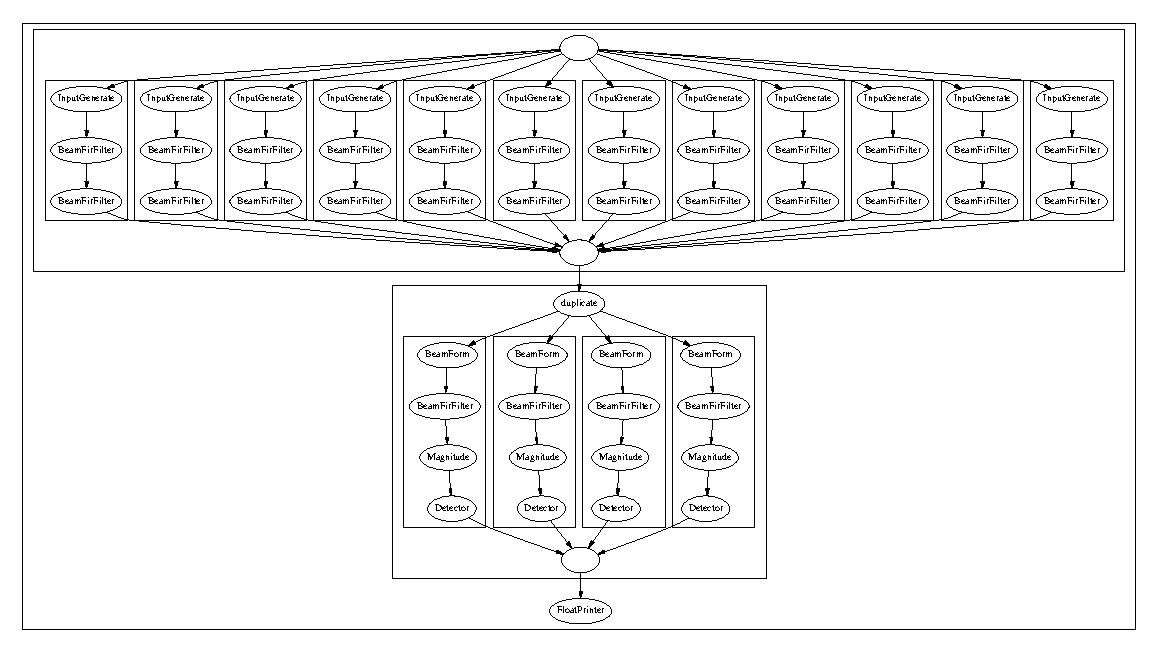
\includegraphics[width=5.0in]{figures/beamformer.eps}
  \caption{A DSP block diagram of the application Beamformer}
  \label{fig:block-diagram}
\end{figure}

    Blocks can be characterized in various ways. The simplest characterization
of blocks is a \textit{linear} block, defined as a module that
outputs a linear combination of its inputs plus a constant term. A
linear block can be represented by a matrix relating inputs to
outputs and a vector of constants. The next simplest
characterization of blocks is \textit{linear state-space}. Such a
block uses a set of state variables. The output of this block is a
linear combination of its inputs and state variables. In addition,
the state variables are updated by a linear combination of
themselves and inputs.  A linear state-space block can be
represented by four independent matrices.

    A linear state-space characterization is more general than a
linear characterization - all linear blocks are also linear
state-space blocks, but the converse is not true. The intuitive
reason for this fact is that a linear block is memoryless, meaning
the outputs only depend on current inputs. However, a linear
state-space block has memory in the form of state variables, so
the outputs depend on current inputs and past inputs.

    We will perform analysis and optimization of DSP applications at
the linear state-space level. We choose this representation
because it models a wide class of applications or parts of
applications, and it is simple to work with.

    Our work with state-space representations will be done in the
context of StreamIt, a programming language designed for streaming
applications \cite{streamitcc}.  StreamIt allows users to create
their own blocks, but limits the way these blocks can be
connected. We perform the following steps on a StreamIt program:

\begin{enumerate}
\vspace{\itemshrink} \item Examine each block and determine whether or not it can be
characterized as linear state-space. If it can, extract the
appropriate state-space representation.

\vspace{\itemshrink} \item Combine connected blocks that each have a state-space
representation, using an appropriate set of rules depending on the
type of connection.

\vspace{\itemshrink} \item Optimize representations through the use of state-space
transformations.

\vspace{\itemshrink} \item Convert the state-space representation(s) back to StreamIt
code.
\vspace{\itemshrink} \end{enumerate}

\mysubsection{Organization}

    The rest of this paper is organized as follows.  In Section 2 we
provide background information about StreamIt and formal linear
and linear state-space models.  Section 3 is devoted to
state-space analysis of StreamIt programs (Items 1, 2, and 4).
Section 4 describes optimizations (Item 3). In Section 5 we
discuss our implementation and results.  Section 6 details related
work, and Section 7 concludes.
